\subsection{Programas utilizados}

Para llevar a cabo las distintas etapas de pre-procesamiento, 
simulaci\'on y 
post-procesamiento, se utilizaron
los siguientes programas:

\begin{itemize}
    \item Quantum ESPRESSO : Paquete de simulaci\'on
    \item VESTA : Generaci\'on y visualizaci\'on de la estructura at\'omica 
    utilizada en la simulaci\'on
    \item XCrySDen : Generaci\'on del camino de puntos K para el c\'alculo de 
    la estructura de bandas de energ\'ia. Adem\'as permite revisar que la 
    estructura del archivo de control de Quantum ESPRESSO sea el adecuado.
    \item Veusz : Programa para generar gr\'aficas
    \item Scripts : Scripts espec\'ificos desarrollados exclusivamente para el 
    presente trabajo en python y shell para automatizar procesos.
\end{itemize}

\noindent Dentro del paquete de simulaci\'on Quantum ESPRESSO se utilizaron los 
siguientes paquetes espec\'ificos:

\begin{itemize}
    \item pw.x : Realiza el c\'alculo de autoconsistencia y el c\'alculo de 
    bandas de energ\'ia.
    \item bands.x : Extrae la informaci\'on correspondiente a cada una 
    de las bandas de energ\'ia, desde los archivos de salida producidos por pw.x
    \item projwfc.x : Realiza el c\'alculo de densidad de estados total y 
    parcial.
    \item plotband.x : Grafica las bandas de energ\'ia a partir de lo obtenido 
    con bands.x
    \item pp.x : Extrae los datos correspondientes a la densidad de carga, a 
    partir de lo obtenido con pw.x
    \item plotrho.x : Grafica la densidad de carga a partir de lo obtenido con 
    pp.x
\end{itemize}

\subsection{Proceso de simulaci\'on}

El flujo de trabajo consta de una serie de pasos que pueden ser agrupados en 
tres grupos.

\begin{itemize}
    \item Preprocesamiento.
    \item Simulaci\'on.
    \item Postprocesamiento.
\end{itemize}

\noindent Cada uno de estos tres grupos se conforma de una serie de pasos, que 
se listan 
a continuaci\'on.

\begin{enumerate}
    \item \textbf{Preprocesamiento:}
        \begin{itemize}
            \item Optimizaci\'on de la energ\'ia de corte.
            \item Optimizaci\'on del n\'umero de puntos K.
            \item Generacion de las estructuras cristalinas con los diferentes 
            arreglos antiferromagn\'eticos
            \item Relajaci\'on de las estructuras cristalinas.
        \end{itemize}
    \item \textbf{Simulaci\'on:}
        \begin{itemize}
            \item C\'alculo autoconsistente con pw.x
            \item C\'alculo de la densidad de carga con pp.x
            \item C\'alculo no autoconsistente con pw.x
            \item C\'alculo de la densidad de estados total y parcial con 
            projwfc.x
            \item C\'alculo de las bandas de energ\'ia con pw.x
            \item Obtenci\'on de los datos de cada una de las bandas de 
            energ\'ia con bands.x
        \end{itemize}
    \item \textbf{Postprocesamiento:}
        \begin{itemize}
            \item Procesamiento de los archivos obtenidos con projwfc.x 
            utilizando el script de python suma\_pdos.py para luego graficar 
            las densidades de estado.
            \item Procesamiento de los archivos obtenidos con bands.x 
            utilizando el script de python banda\_plot.py para luego graficar 
            las bandas.
        \end{itemize}
\end{enumerate}

\subsection{Arreglos antiferromagn\'eticos}

Para realizar la simulaci\'on se dispuso la estructura cristalina de ambos 
materiales en varios arreglos antiferromagn\'eticos. Esto se logro colocando 
los espines de los \'atomos de hierro y cromo del $BiFeO_{3}$ y $YCrO_{3}$ 
respectivamente, en direcciones paralelas y antiparalelas entre ellos de 
acuerdo a los tipos de arreglos antiferromagn\'eticos escogidos. 
En el caso del $BiFeO_{3}$ se utilizaron los arreglos antiferromagn\'eticos 
tipo A y G, los cuales se pueden observar en forma esquem\'atica en la figura 
\ref{arreglos_BFO}.

\begin{figure}[H]
    \centering
    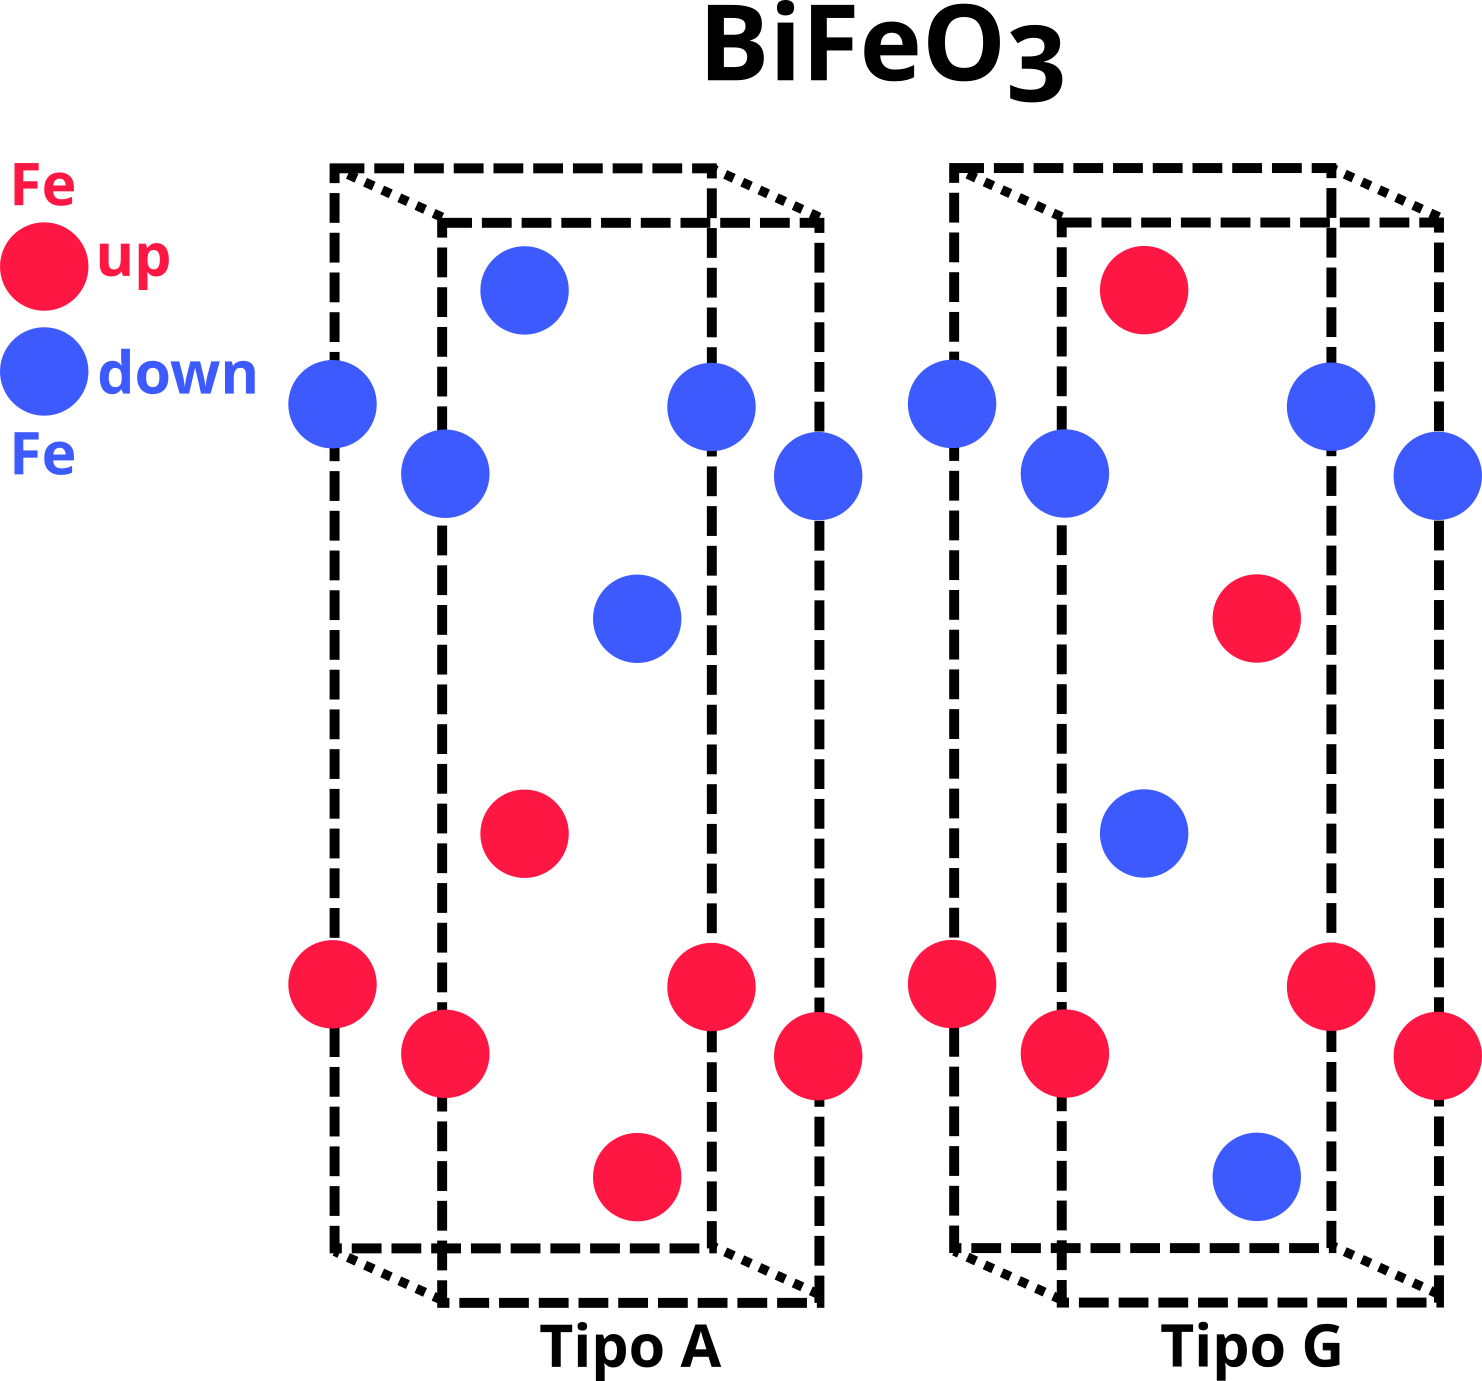
\includegraphics[width=0.5\textwidth]{contenido/marco_teorico/metodologia/img_metodologia/BFO_unido.png}
    \caption[Arreglos antiferromagn\'eticos $BiFeO_{3}$]{Arreglos 
        antiferromagn\'eticos para el $BiFeO_{3}$ se muestran solo los \'atomos 
        de hierro por claridad}
    \label{arreglos_BFO}
\end{figure}

\noindent En el caso del $YCrO_{3}$ se utilizaron los arreglos 
antiferromagn\'eticos tipo 
A, C y G, los cuales se pueden observar en forma esquem\'atica en la figura 
\ref{arreglos_YCO}.

\begin{figure}[H]
    \centering
    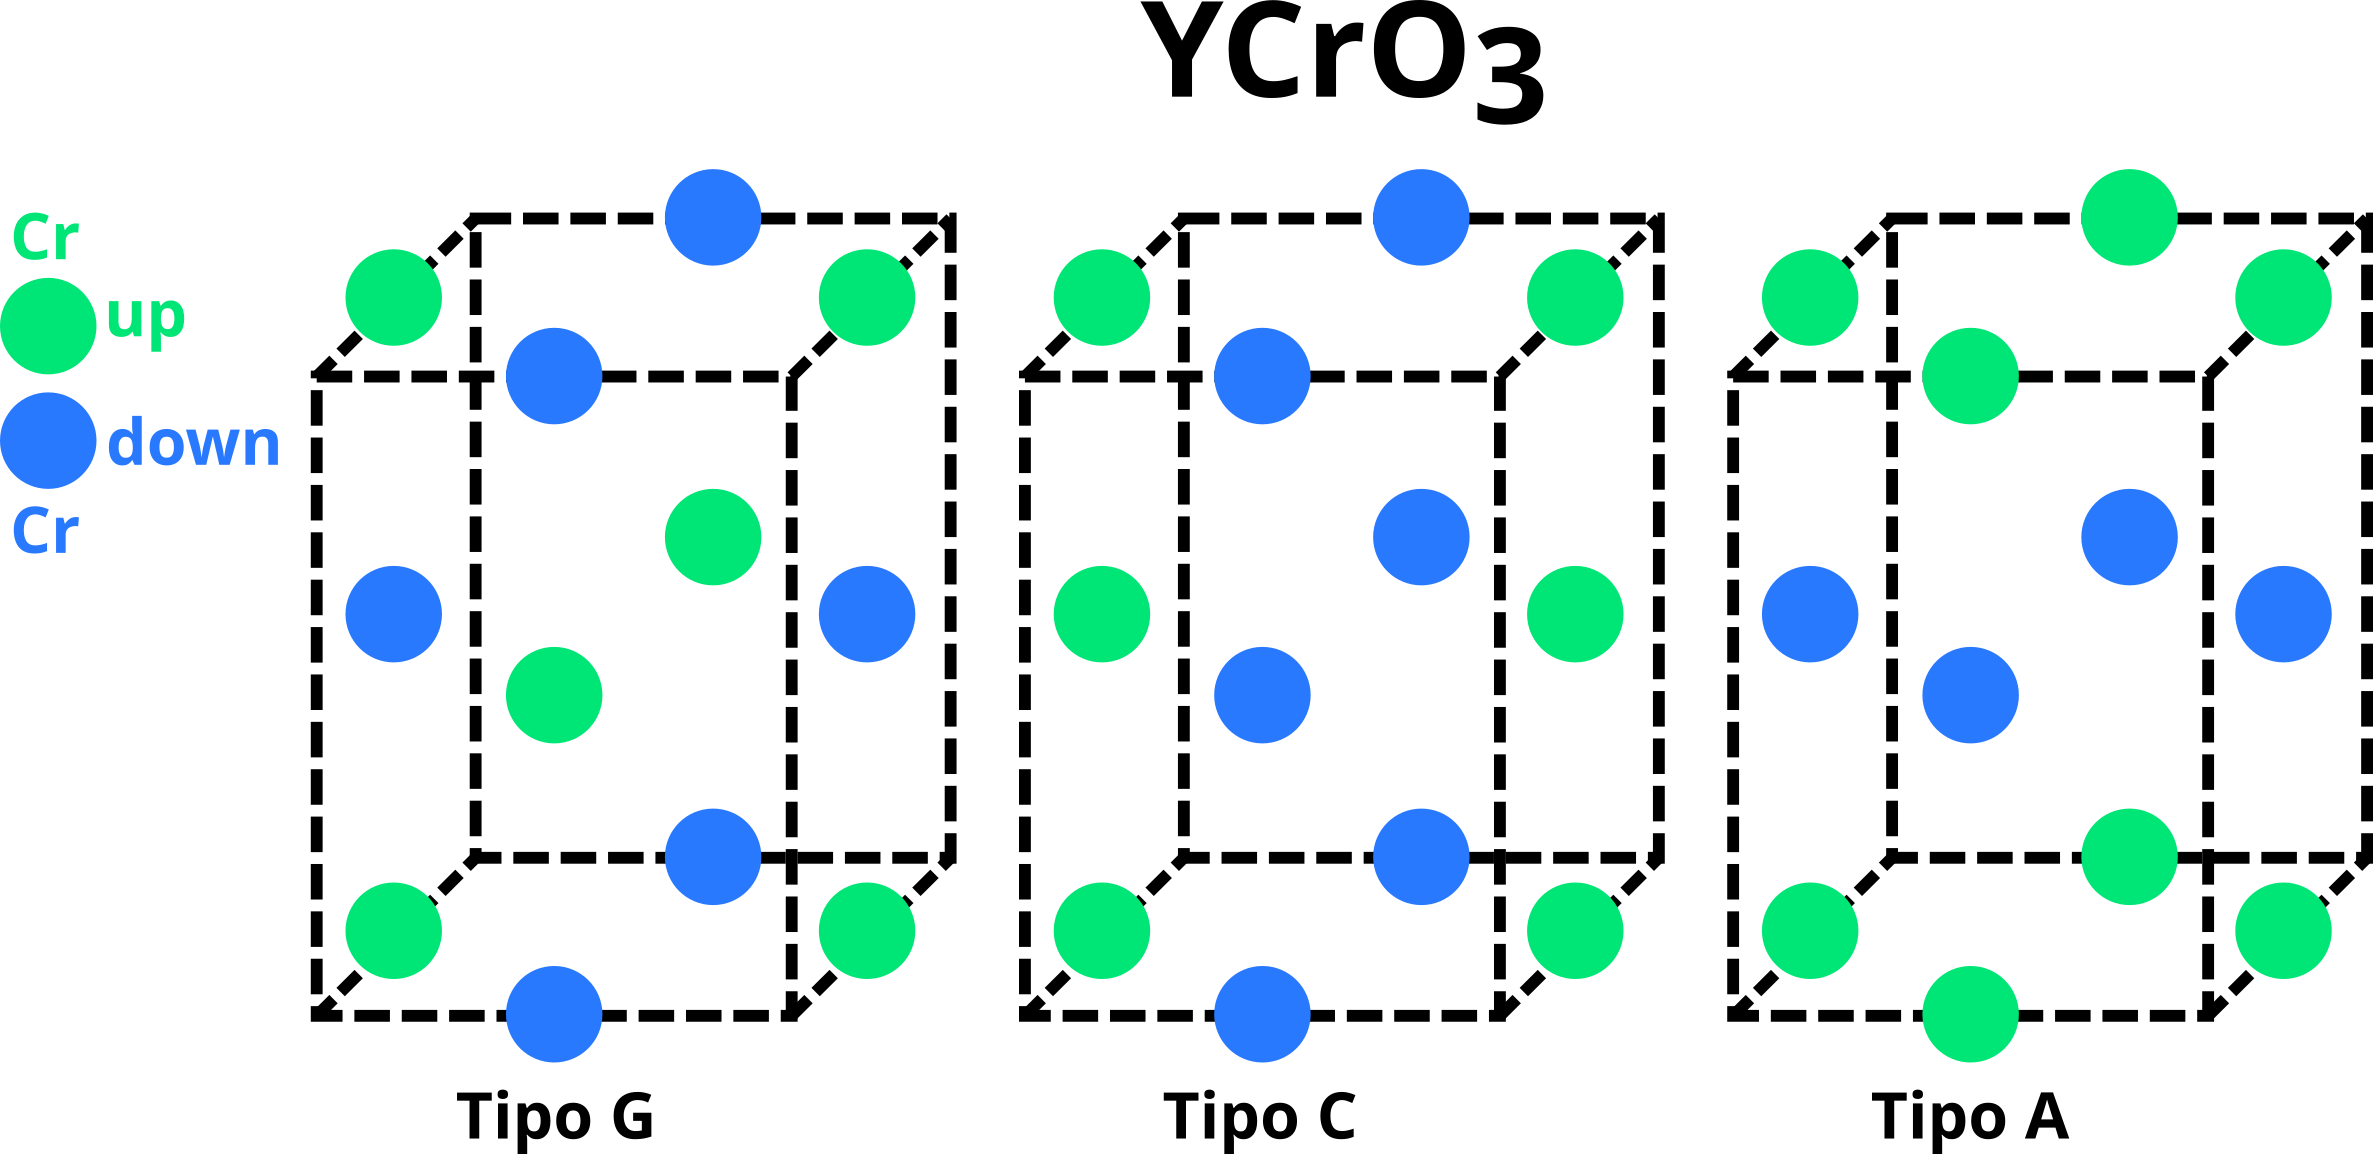
\includegraphics[width=0.6\textwidth]{contenido/marco_teorico/metodologia/img_metodologia/YCO_unido.png}
    \caption[Arreglos antiferromagn\'eticos $BiFeO_{3}$]{Arreglos 
        antiferromagn\'eticos para el $YCrO_{3}$ se muestran solo los \'atomos 
        de cromo por claridad}
    \label{arreglos_YCO}
\end{figure}